\documentclass[11pt,twoside,a4paper]{article}
\usepackage{fullpage}
\usepackage{graphicx}
\usepackage{amsmath}
\usepackage{listings}
\usepackage{color} %red, green, blue, yellow, cyan, magenta, black, white
\definecolor{mygreen}{RGB}{28,172,0} % color values Red, Green, Blue
\definecolor{mylilas}{RGB}{170,55,241}

\title{Wettbewerb Matrixoptik}
\author{Alain Better than Big Keller}

\begin{document}
	\maketitle
	\section{Analyse Aufgabenstellung}
	Ziel der Aufgabe ist, ein Optisches System aus vier bi-konvexen Linsen zu analysieren und mit Hilfe der Matrixoptik zu berechnen. \\
	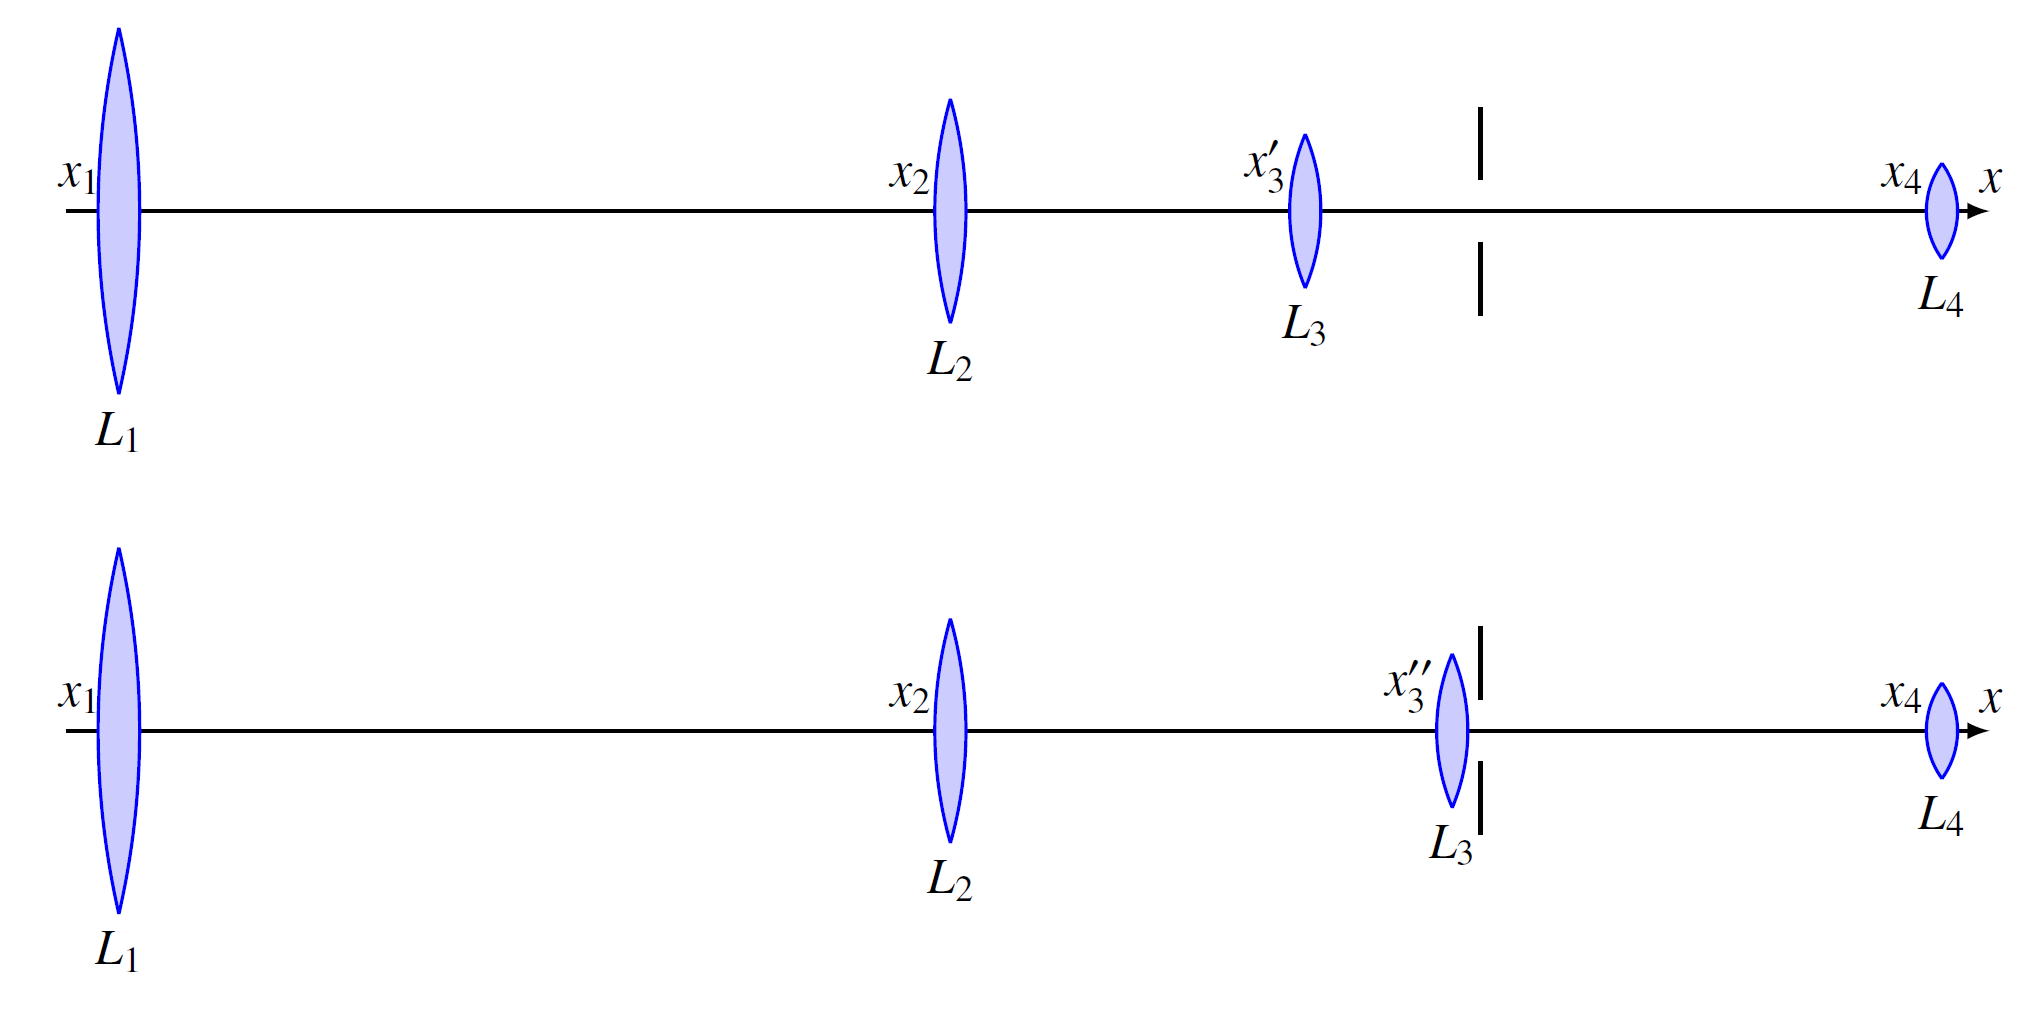
\includegraphics[scale=.25]{./system.PNG}
	\begin{table}
		\centering
		\begin{tabular}{lllll}
			Brechungsindex n & Linse & Krümmungsradius R [mm]& Dicke d [mm] & Position x [mm] \\
			1.5 & \(L_{1}\) & 78.672364 & 4 & \(x_{1}\) = 0 \\
			1.5 & \(L_{2}\) & 39.603940 & 3 & \(x_{2}\) = 80 \\
			1.5 & \(L_{3}\) & 19.013503 & 3 & \(x'_{3}\) = \(x_{2} + 20 * (1+\frac{1}{\sqrt{2}})\)  \\
			1.5 & \(L'_{3}\) & 19.013503 & 3 & \(x''_{3}\) = \(x_{2} + 20 * (1+\sqrt{2})\) \\
			1.5 & \(L_{4}\) & 7.8042263 & 3 & \(x_{4}\) = Unbekannt \\
		\end{tabular}
	\end{table} \\
	Das ganze Optische System, wie in der Darstellung dargestellt, mit den Daten der Tabelle 1 lässt sich mit Hilfe der Matrixoptik berechnen. Das Verhalten eines Lichtstrahles, welcher durch dieses Optische System geht, lässt sich mit einer Transfermatrix beschreiben. Durch diese Matrix lässt sich der Ausgangswinkel und -Höhe eines einfallenden Lichtstrahles mit bekanntem Einfallswinkel, und -Höhe berechnen. Da in dieser Aufgabe das System nur angenähert berechnet wird, wird mit \(sin(\theta) = \theta\) gerechnet.
	\begin{equation} \label{Transfermatrix1}
	\begin{pmatrix}
	A & B \\
	C & D
	\end{pmatrix}
	\quad
	\begin{pmatrix}
	y_{1}\\
	\theta_{1}
	\end{pmatrix}
	\quad
	=
	\quad
	\begin{pmatrix}
	y_{2}\\
	\theta_{2}
	\end{pmatrix}
	\end{equation}
	\ref{Transfermatrix1} Beispiel einer Transfermatrix multipliziert mit dem Lichtstrahl-Vektor wobei y die Höhe über der optischen Achse (x in der Abbildung) des Lichtstrahles und \(\theta\) den Winkel zur optischen Achse beschreibt \\
	
	Das Ziel ist es eine solche Transfermatrix dieses optischen Systems zu berechnen, da sich mit dieser die gefragten Werte berechnen lassen. 
	\section{Aufgabe 1 und 2}
	In dieser Aufgabe müssen wir die Position der letzten Linse \(L_{4}\) so berechnen, dass das System scharf abbildet. Dies ist, wie in der Aufgabenstellung schon beschrieben, der Fall wenn horizontal einfallende Strahlen wieder Horizontal austreten. Allgemein kann man sagen, dass eintretende Strahlen, welche zueinander parallel sind, wieder zueinander parallel austreten.
	Das bedeutet für die Transfermatrix, wenn ein Strahl mit \(\theta_{1} = 0\) und \(y_{1} \neq 0\) in das System kommt dieser wieder mit \(\theta_{2} = 0\) austritt. Anders ausgedrückt: 
	\begin{equation} \label{scharfAbb}
	\begin{aligned}[C]
		C * y_{1} + D * \theta_{1} = 0 \nonumber \\
		\textrm{Da \(\theta_{1} = 0\) und \(y_{1} \neq 0\) kann man vereinfachen:} \nonumber\\
		C = 0
	\end{aligned}
	\end{equation}
	Das heisst mit der Position C in der Transfermatrix können wir die gesuchte Position der Linse 4 berechnen. \\
	Damit wir die die oben genannte Rechnung durchführen können benötigen wir die Transfermatrix \(T\), berechnet mit der unbekannten \(x_{4}\).  
	\subsection{Berechnung von T}
	Die Transfermatrix des gesamten Systems besteht aus den jeweiligen Transfermatrizen der einzelnen Linsen und Räume zwischen den Linsen. Für jeden Raum, und Mediumswechsel, welcher ein Lichtstrahl durchquert gibt es eine Transfermatrix. In verkehrter Reihenfolge, wie sich der Lichtstrahl bewegt, multipliziert ergeben sie die Transfermatrix des gesamten Systems.
	\begin{equation} \label{tMatrixRaum}
	T_{l} = 
	\begin{pmatrix}
	1 & l \\
	0 & 1
	\end{pmatrix}
	\end{equation}
	\begin{equation*}
	\begin{aligned}
	T_{a1} \approx
	\begin{pmatrix}
	1 & 76.5 \\
	0 & 1
	\end{pmatrix} &
	&
	T_{a2}\textrm{ (\(L_{3}\) bei \(x'_{3}\))} \approx
	\begin{pmatrix}
	1 & 31.1421 \\
	0 & 1
	\end{pmatrix} \\
	T_{a22}\textrm{ (\(L_{3}\) bei \(x''_{3}\))} \approx
	\begin{pmatrix}
	1 &    45.2843 \\
	0 & 1
	\end{pmatrix}&
	&
	T_{a3} \approx
	\begin{pmatrix}
	1 & x_{4} \\
	0 & 1
	\end{pmatrix}
	\end{aligned}
	\end{equation*}
	\ref{tMatrixRaum} Matrix um einen Lichtstrahl, welcher sich durch einen Raum aus einem Medium bewegt, beschriebt. \(l\) ist die Länge dieses Raumes.
	\begin{equation} \label{tMatrixBrechung}
		B(n_{1},n_{2},R) = 
		\begin{pmatrix}
		1 & 0 \\
		\frac{1}{R}(\frac{n_{1}}{n_{2}}-1) & \frac{n_{1}}{n_{2}}
		\end{pmatrix}
	\end{equation}
	\ref{tMatrixBrechung} Transfermatrix um eine Brechung an einer gekrümmten Oberfläche zu berechnen. \(n_{1}\) ist der Brechungsindex des Mediums von dem der Lichtstrahl kommt und \(n_{2}\) derjenige des Mediums in das der Lichtstrahl geht. Der Radius R ist bei einem Übergang an einer konvexen Oberfläche positiv und bei einer konkaven negativ. Die Brechungsmatrix basiert auf dem Brechungsgesetz von Snellius.  \\
	Will man nun beschreiben wie sich ein Lichtstrahl durch eine Linse bewegt braucht man drei Transfermatrizen, die Brechung beim eintritt, wie sich der Strahl durch die Linse bewegt, und die Brechung beim Austritt. Die Transfermatrix erfolgt nun aus der Multiplikation dieser drei Matrizen. Für eine symmetrische bi-konvexe Linse sieht das wie folgt aus: 
	\begin{equation*} \label{SymmLinse}
	B(n_{2},n_{1},-R)*T_{l}*B(n_{1},n_{2},R) = T
	\end{equation*}
	\begin{equation*}
	\begin{aligned}
	T_{L1} \approx
	\begin{pmatrix}
	0.9831 & 2.6667 \\
	-0.0126 & 0.9831
	\end{pmatrix} &
	&
	T_{L2} \approx
	\begin{pmatrix}
	0.9831 & 2.6667 \\
	-0.0126 & 0.9831
	\end{pmatrix} \\
	T_{L3} \approx
	\begin{pmatrix}
	0.9831 & 2.6667 \\
	-0.0126 & 0.9831
	\end{pmatrix}&
	&
	T_{L4} \approx
	\begin{pmatrix}
	0.9831 & 2.6667 \\
	-0.0126 & 0.9831
	\end{pmatrix}
	\end{aligned}
	\end{equation*}
	Hat man nicht nur eine sondern zwei Linsen mit einem Abstand \(a\) dazwischen muss man diesen in die Rechnung miteinbeziehen. Die Rechnung würde dann wie folgt aussehen: 
	\begin{equation} \label{SymmLinse}
	T_{2}*T_{a}*T_{1} = T
	\end{equation}
	Auf das System der Aufgabe angewandt sieht die Berechnung der Transfermatrix so aus: 
	\begin{equation} \label{TLinsSys}
	T = T_{L4}T_{a3}T_{L3}T_{a2}T_{L2}T_{a1}T_{L1}
	\end{equation}
	\begin{equation*}
	\begin{aligned}
	\textrm{T für \(L_{3}\) bei \(x'_{3}\) } & T \approx
	&
	\begin{pmatrix}
	0.0075\,x_4 -0.3388 & 30.6137-2.9219\,x_4 \\
	0.0565-0.0010\,x_4  & 0.4019\,x_4 -8.0548
	\end{pmatrix}\\
	\textrm{T für \(L_{3}\) bei \(x''_{3}\) } & T' \approx
	&
	\begin{pmatrix}
	0.0156\,x'_4 -0.4693 & 20.5528-2.3011\,x'_4 \\
	0.0850-0.0021\,x'_4  & 0.3165\,x'_4 -5.8542
	\end{pmatrix}
	\end{aligned}
	\end{equation*}
	\ref{TLinsSys} Die Matrizen \(T_{a1},T_{a2},T_{a3}\) beschrieben den Abstand zwischen den Linsen. Dabei ist zu beachten, dass bei \(T_{a3}\) die Distanz noch Unbekannt ist, und bei den bekannten Distanzen die Dicken der Linsen subtrahiert werden, um die Distanz zwischen den Linsenoberflächen zu erhalten. Die Matrizen \(T_{L1},T_{L2},T_{L3},T_{L4}\) beschrieben die Transfermatrizen der Linsen. Diese wurden nach dem oben erwähnten Prinzip berechnet, wobei für den Brechungsindex \(a_{1}\) 1 verwendet wurde, da in der Aufgabe die Linsen von Luft, für welches n = 1 gilt, umgeben sind.
	Die Transfermatrix für das System wurde mit einem Matlab Skript berechnet. Die Matrix hat jedoch noch eine Unbekannte, die Distanz zwischen \(L_{3}\) und \(L_{4}\). Diese Unbekannte lässt sich nach dem oben genannten Prinzip Berechnen (die Zahl in Zeile 2 und Spalte 1 muss null sein). \\
	\\
	Löst man die Gleichung für \(x_{4}\) und \(x'_{4}\) auf bekommt man die jeweiligen Abstände zur Linse 3. Addiert man nun die Bekannten Abstände und die Linsendicken, kommt man auf das Ergebnis, dass die Linse 4 nur um  0.8434mm verschoben werden muss, damit das System in beiden Positionen scharf abbildet. Dies ist sogleich die Antwort auf die Zweite Frage. \\
	Position der vierten Linse, wenn die Dritte Linse bei \(x'_{3}\) ist: 171.8567847673568127905970695569mm \\
	Position der vierten Linse, wenn die Dritte Linse bei \(x''_{3}\) ist: 171.01342515747323965389575288258mm \\
	\begin{equation*}
	\begin{aligned}
	T \approx
	&
	\begin{pmatrix}
	0.0718 & -129.2555\\
	0 & 13.9355
	\end{pmatrix}\\
	T' \approx
	&
	\begin{pmatrix}
	0.1488 & -70.8665\\
	0 & 6.7207
	\end{pmatrix}
	\end{aligned}
	\end{equation*}
	\section{Aufgabe 3 und 4}
	Da das Linsensystem bei Position \(x''_{3}\) eine Blende hat, wird die Vergrösserung mit einem Lichtstrahl berechnet, der diese Blende durchquert. Die Blende sorgt dafür, dass nur bestimmte Lichtstrahlen das System durchqueren können. \\
	Um herauszufinden welche Lichtstrahlen die Position (\(x''_{3},0\)) durchqueren brauchen wir eine Transfermatrix, die bis zu diesem Punkt geht, also ohne die vierte Linse und deren Abstand zur dritten Linse.
	Da das System zwei verschiedene Positionen für die dritte Linse erlaubt, wird für jede Position eine Transfermatrix benötigt. 
	\begin{equation*}
	\begin{aligned}
	\textrm{Transfermatrix von \(x_{1}\) bis \(x''_{3}\) für \(L_{3}\) bei \(x'_{3}\) } & T \approx
	&
	\begin{pmatrix}
	-0.2995 & 0.4330\\
	0.0086 & -3.3512
	\end{pmatrix}\\
	\textrm{Transfermatrix von \(x_{1}\) bis \(x''_{3}\) für \(L_{3}\) bei \(x''_{3}\) } & T \approx
	&
	\begin{pmatrix}
	-0.5818 & 31.4878\\
	0.0017 & -1.2401
	\end{pmatrix}
	\end{aligned}
	\end{equation*}
	\subsection{Vergrösserung 1}
	Entscheidend dafür, ob ein Lichtstrahl durch einen bestimmten Punkt geht, ist das Verhältnis zwischen Abstand und Winkel zur optischen Achse. Mit Hilfe der Transfermatrix von \(x_{1}\) nach \(x''_{3}\) und einem Lichtvektor mit Variablen, lässt sich ausrechnen in welchen Verhältnis die beiden Variablen des Lichtvektors sein müssen um die Blende zu durchqueren( Der berechnete Vektor muss einen y-Wert von 0 haben). Das berechnete Verhältnis ist: \(y:\theta \approx 1:0.6916\) Mit dem Ermittelten Ergebnis wurde ein Lichtstrahl erstellt, welcher die Blende durchquert. Die Transfermatrix wird nun mit diesem Multipliziert. \\
	Die Vergrösserung eines Optischen Systems lässt sich mit dem Verhältnis vom Einfallswinkel zum Ausfallswinkel berechnen (Strahlensatz). 
	\begin{equation} \label{vergr}
	\begin{pmatrix}
	T
	\end{pmatrix}
	\quad
	\begin{pmatrix}
	y_{1}\\
	\theta_{1}
	\end{pmatrix}
	\quad
	=
	\quad
	\begin{pmatrix}
	y_{2}\\
	v * \theta_{1}
	\end{pmatrix}
	\end{equation}
	
	\ref{vergr} Lichtvektor multipliziert mit einer Transfermatrix. \(v\) stellt hierbei den Vergrösserungsfaktor dar.  \\
	Zur Berechnung der Vergrösserung wird ein Lichtvektor mit dem berechneten Verhältnis verwendet. Hierbei wird für den Winkel eine Variable, und für den Offset zur optischen Achse eine Funktion(Verhältnis) des Winkels genommen, da sich der Winkel am Ende wegkürzen lässt. Die Transfermatrix des gesamten Systems wird nun mit diesem Vektor multipliziert. Vom berechneten Vektor wird nun der Wert in der zweiten Spalte durch den Winkel geteilt, und man bekommt das Verhältnis, welches auch die Vergrösserung darstellt.
	\begin{equation}
	\begin{pmatrix}
	T
	\end{pmatrix}
	\begin{pmatrix}
	1.4459\,\theta_1 \\
	\theta_1 
	\end{pmatrix}
	\approx
	\begin{pmatrix}
	-129.1517\,\theta_1 \\
	13.9355\,\theta_1
	\end{pmatrix}
	\end{equation}
	Anhand des Vektors kann man Ablesen, dass der Vergrösserungsfaktor ungefähr 13.9355 ist.
	\subsection{Vergrösserung 2}
	Um die Vergrösserung des Systems zu berechnen wenn die dritte Linse bei der Position \(x''_{3}\) ist, lässt sich fast gleich wie die vorherige Vergrösserung berechnen. Der einzige unterschied ist die Transfermatrix für die Berechnung eines Lichtstrahles, der durch den Punkt (\(x''_{3},0\)) geht. Da sich die Blende an der Position \(x''_{3}\) befindet, ist sie in diesem Fall in der Mitte der dritten Linse. Dafür wird für die Dritte Linse eine zusätzliche Transfermatrix berechnet, welche die halbe Linse beschreibt. Mit dieser wird dann die Transfermatrix von \(x_{1}\) bis \(x''_{3}\) berechnet. Berechnet man nun wieder das Verhältnis zwischen Winkel und Höhe eines Lichtstrahles kommt man auf das Ergebnis: \(y_{1} : \theta_{1} \approx 1:0.01848\) Die restlichen Schritte sind die selben wie schon für die erste Vergrösserung angewendet wurden.
		\begin{equation}
	\begin{pmatrix}
	T
	\end{pmatrix}
	\begin{pmatrix}
	54.1189\,\theta_2 \\
	\theta_2  
	\end{pmatrix}
	\approx
	\begin{pmatrix}
	-62.8139\,\theta_2 \\
	6.7207\,\theta_2
	\end{pmatrix}
	\end{equation}
	Auch hier kann man den Vergrösserungsfaktor im Rechten Vektor ablesen. Er beträgt ungefähr: 6.7207
	\subsection{Unterschied zum Keplerteleskop}
	Ein wesentlicher Unterschied, welcher beim berechnen des Systems aufgefallen ist die Vergrösserung. Ein Kepler-Teleskop hat eine Negative Vergrösserung, das heisst, das Bild ist "auf dem Kopf". Bei unserem System ist die Vergrösserung Positiv, also wird das Bild in der gleichen Ausrichtung Projiziert. Dies kann auch mit einem parallel zur optischen Achse einfallenden Strahl gezeigt werden. Dieser verlässt das System wieder auf der selben Seite, wie er eingefallen ist. Dieser Unterschied ist für den Gebrauch des Systems nützlich, da die Ausrichtung auf ein Ziel natürlicher ist.
	\begin{table}
		\centering
		\begin{tabular}{ll}
			\(x_{4}\) wenn \(x_{3} = x'_{3}\) & 171.8567847673568127905970695569mm \\
			\(x_{4}\) wenn \(x_{3} = x''_{3}\) & 171.01342515747323965389575288258mm \\
			Verschiebung von \(L_{4}\) bei verschiebung von \(L_{3}\) & 0.84335960988357313670131667432176mm\\
			Vergrösserung wenn Linse 3 bei \(x'_{3}\) & 13.935473269228034340293197061854 \\
			Vergrösserung wenn Linse 3 bei \(x''_{3}\) & 6.7206696976667773330755532059945 \\
			Unterschied zu Kepler-Teleskop & Das System gibt das Bild in der selben Ausrichtung aus \\
		\end{tabular}
	\end{table} \\

\lstset{language=Matlab,%
	%basicstyle=\color{red},
	breaklines=true,%
	morekeywords={matlab2tikz},
	keywordstyle=\color{blue},%
	morekeywords=[2]{1}, keywordstyle=[2]{\color{black}},
	identifierstyle=\color{black},%
	stringstyle=\color{mylilas},
	commentstyle=\color{mygreen},%
	showstringspaces=false,%without this there will be a symbol in the places where there is a space
	numbers=left,%
	numberstyle={\tiny \color{black}},% size of the numbers
	numbersep=9pt, % this defines how far the numbers are from the text
	emph=[1]{for,end,break},emphstyle=[1]\color{red}, %some words to emphasise
	%emph=[2]{word1,word2}, emphstyle=[2]{style},    
}


\section*{Matlab Code}

\lstinputlisting{MatrixOptik.m}



\end{document}
